
The proof of this theorem will be given in Section~\ref{ss:proof1}. We make use of the refinement order on set compositions to show that the set $\mathcal{C}_{\alpha,x}^{\beta,y}$ has a unique minimum. We will use this fact along with other properties to construct sign reversing involutions on $\mathcal{C}_{\alpha,x}^{\beta,y}$ and the result will follow once we understand the fixed points of such involutions.

%%%%%%%%%%%%%%
%% REFINEMENT ORDER 
%%%%%%%%%%%%%%
\subsection{Minimal element of \texorpdfstring{$\mathcal{C}_{\alpha,x}^{\beta,y}$}{C alpha,x beta,y}}\label{ss:refinementonC}
Given set compositions $A=(A_1,\ldots,A_k)$ and $B=(B_1,\ldots,B_\ell)$ on a set $I$, 
we say that $A$ \emph{refines} $B$, and we write $A\le B$, if the parts of $B$ are unions of consecutive parts of $A$. For example
 $$A = \big(\{1,4\},\{2\},\{5,7\},\{3\},\{9\},\{6,8\}\big) \le \big(\{1,4\},\{2,3,5,7\},\{6,8,9\}\big)=B$$
but $A$ does not refine $\big(\{1,4,5,7\},\{2\},\{3\},\{9\},\{6,8\}\big)$. Denote by $(\mathcal{P}_I,\leq)$ the poset of set compositions of $I$, ordered by refinement.
In what follows we will write $(14,2,57,3,9,68)$ instead of $\big(\{1,4\},\{2\},\{5,7\},\{3\},\{9\},\{6,8\}\big)$. Consider the order $\le$ restricted to the set $\mathcal{C}_{\alpha,x}^{\beta,y}$.

\begin{lemma}\label{le:min}
If $\mathcal{C}_{\alpha,x}^{\beta,y}\ne\emptyset$, then there is a unique minimal element in $(\mathcal{C}_{\alpha,x}^{\beta,y},\le)$.
\end{lemma}
\begin{proof} Suppose that $A=(A_1,\ldots,A_k)$ and $B=(B_1,\ldots,B_\ell)$ are minimal in $\in \mathcal{C}_{\alpha,x}^{\beta,y}$ and $A\neq B$. We have that $\alpha_A=\beta=\alpha_B$ and $x_A=y=x_B$. Since $\alpha_A=\beta$, the parts of $A$ appear consecutively in $\beta$ and the same is true for the parts of $B$. For example if $\alpha=abcdef$ and $\beta=bcfade$, then for $A=(bc,f,ad,e)$ and $B=(bc,f,a,de)$ we have $\alpha_A=\alpha_B=\beta$.

 Let $1\le i\le k$ be the smallest index such that $A_i\ne B_i$, and assume without loss of generality that $|A_i|>|B_i|$. If $i=k$ then $B$ refines $A$ and this is a contradiction. Hence we assume that $i<k$ and we now build a composition $C$ that refines $A$ such that $C\in \mathcal{C}_{\alpha,x}^{\beta,y}$, which will contradict again the minimality of $A$. Since $\alpha_A=\alpha_B$ our choice of $i$ implies that $B_i\subset A_i$.
Let $U=A_i\setminus B_i$. We claim that for $C=(A_1,\ldots,A_{i-1},B_i,U,A_{i+1},...,A_k)$
\begin{enumerate}[(a)]
\item %[(a)]
\label{proof_of_2-2_a} $C<A$ 
\item %[(b)]
\label{proof_of_2-2_b} $\alpha_C=\alpha_A=\beta$
\item %[(c)]
\label{proof_of_2-2_c} $x_C=x_A=y$
\end{enumerate}
Items~\ref{proof_of_2-2_a} and~\ref{proof_of_2-2_b} are straightforward. For~\ref{proof_of_2-2_c} we show that for some $P$ and $T$ we get
\begin{equation}\label{eq:xCisxA}
x_A=\mu_{P,T}\Delta_{P,T}\mu_A\Delta_A(x)=\mu_C\Delta_C(x).
\end{equation}

Let $P=B_1\cup\cdots\cup B_i$ and $T=B_{i+1}\cup\cdots\cup B_\ell$.
We claim that
\begin{equation}\label{eq:Tcutx}
 x_B=\mu_{P,T}\Delta_{P,T}(x_B).
\end{equation}
To see this, we use the associativity of $\mu$ to write $\mu_B=\mu_{P,T}(\mu_{B_1,\ldots,B_i}\otimes\mu_{B_{i+1},\ldots,B_\ell})$. Also, let $Q=R=\emptyset$ in the compatibility relation~\eqref{e:comp}, we get $A_1=P$, $A_2=T$ and 
 $$\Delta_{P,T}\mu_{P,T}=\Id_P\otimes \Id_T,$$
where $\Id_A$ denotes the identity map on $A$. Hence equation~\eqref{eq:Tcutx} follows from
 $$
 \begin{aligned}
 \mu_{P,T}\Delta_{P,T}(x_B)&=\mu_{P,T}\Delta_{P,T}\mu_{P,T}(\mu_{B_1,\ldots,B_i}\otimes\mu_{B_{i+1},\ldots,B_\ell})\Delta_B(x)\\
 &=\mu_{P,T}(\mu_{B_1,\ldots,B_i}\otimes\mu_{B_{i+1},\ldots,B_\ell})\Delta_B(x)=\mu_B\Delta_B(x)=x_B.
 \end{aligned} 
 $$
Using again~\eqref{eq:Tcutx} and the fact that $x_A=x_B$ we show the first equality in~\eqref{eq:xCisxA}:
\begin{equation}\label{eq:TcutS}
 x_A=\mu_{P,T}\Delta_{P,T}(x_A)=\mu_{P,T}\Delta_{P,T}\mu_A\Delta_A(x).
\end{equation}
 Now let $P'=A_1\cup\cdots\cup A_{i-1}$, $Q'=\emptyset$, $R'=B_i $ and $T'=T$ in the compatibility relation~\eqref{e:comp}:
 $$
 \begin{aligned}
 \Delta_{P,T}\mu_A &\Mk= \Mk\Delta_{P'\cup R',T'}\mu_{P',R'\cup T'}(\mu_{A_1,\ldots,A_{i-1}}\otimes \mu_{A_i,\ldots,A_k})\\
 &\Mk=\Mk(\mu_{P',R'}\otimes \Id_{T'})(\Id_{P'}\otimes\Delta_{R',T'})(\mu_{A_1,\ldots,A_{i-1}}\otimes \mu_{A_i,\ldots,A_k})\\
 &\Mk=\Mk(\mu_{P',R'}\Mk\otimes \Mk\Id_{T'})(\mu_{A_1,\ldots,A_{i-1}}\Mk\otimes\Mk\Id_{R'}\Mk\otimes\Mk\Id_{T'})
 (\Id_{A_{1}} \Mk\otimes\Mk\cdots\Mk\otimes \Mk\Id_{A_{i-1}}\Mk\otimes\Mk\Delta_{R',T'}\mu_{A_i,\ldots,A_k}).\\
 \end{aligned}
 $$
 We now expand $\Delta_{R',T'}\mu_{A_i,\ldots,A_k}$ using similar manipulations. Let $T''=A_{i+1}\cup\cdots\cup A_k$,
 $$
 \begin{aligned}
 \Delta_{R',T'}\mu_{A_i,\ldots,A_k} &= \Delta_{B_i , U\cup T''}\mu_{B_i\cup U,T''}(\Id_{A_i}\otimes \mu_{A_{i+1},\ldots,A_k})\\
 &=(\Id_{B_i}\otimes \mu_{U,T''})(\Delta_{B_i,U}\otimes\Id_{T''})(\Id_{A_i}\otimes \mu_{A_{i+1},\ldots,A_k})\\
 &=(\Id_{B_i}\otimes \mu_{U,T''})(\Id_{B_i}\otimes \Id_U\otimes \mu_{A_{i+1},\ldots,A_k})(\Delta_{B_i,U}\otimes\Id_{A_{i+1}}
 \otimes\cdots\otimes \Id_{A_k})\\
 &=(\Id_{B_i}\otimes \mu_{U,A_{i+1},\ldots,A_k})(\Delta_{B_i,U}\otimes\Id_{A_{i+1}} \otimes\cdots\otimes \Id_{A_k}).\\
 \end{aligned}
 $$
Remark that since $R'=B_i$,
 $$
 \begin{aligned}
 \mu_C&=\mu_{P,T}(\mu_{A_1,\ldots,A_{i-1},B_i}\otimes \Id_{T'})(\Id_{A_{1}} \otimes\cdots\otimes \Id_{A_{i-1}}\otimes\Id_{B_i}\otimes \mu_{U,A_{i+1},\ldots,A_k})\\
 &=\mu_{P,T}(\mu_{P',R'}\otimes \Id_{T'})(\mu_{A_1,\ldots,A_{i-1}}\otimes\Id_{R'}\otimes\Id_{T'})
\\ 
&\hspace*{55mm} (\Id_{A_{1}} \otimes\cdots\otimes \Id_{A_{i-1}}\otimes\Id_{B_i}\otimes \mu_{U,A_{i+1},\ldots,A_k})\\
 \end{aligned}
 $$
 and 
 $$\Delta_C=(\Id_{A_{1}} \otimes\cdots\otimes \Id_{A_{i-1}}\otimes\Delta_{B_i,U}\otimes\Id_{A_{i+1}} \otimes\cdots\otimes \Id_{A_k})\Delta_A.$$
 Making use of the expressions given above for $\Delta_{P,T}\mu_A$, and comparing with $\mu_C\Delta_C$ we get
 $$x_A=\mu_{P,T}(\Delta_{P,T}\mu_A)\Delta_A(x)=\mu_C\Delta_C(x)=x_C.$$
We conclude that the composition $C$ satisfies (a), (b) and (c) contradicting the choice of $A$, hence we must have a unique minimal element in $(\mathcal{C}_{\alpha,x}^{\beta,y},\le)$.
\end{proof}

For the rest of this section, let $\alpha,\beta,x$ and $y$ be fixed and let $\Lambda=(\Lambda_1,\Lambda_2,\ldots,\Lambda_m)$ be the minimum of $\mathcal{C}_{\alpha,x}^{\beta,y}\ne \emptyset$.
For any $A\in\mathcal{C}_{\alpha,x}^{\beta,y}$ let $[\Lambda,A]$ denote the interval $\big\{ B\models I : \Lambda\le B\le A\big\}\subseteq \mathcal{P}_I$. A priori, this interval does not need to be contained in $\mathcal{C}_{\alpha,x}^{\beta,y}$, but the following lemma shows that this is indeed the case.

\begin{lemma}\label{le:lowerideal}
If $\mathcal{C}_{\alpha,x}^{\beta,y}\ne\emptyset$, then for any $A\in\mathcal{C}_{\alpha,x}^{\beta,y}$ we have that 
$[\Lambda,A]\subseteq \mathcal{C}_{\alpha,x}^{\beta,y}$.
\end{lemma}

\begin{proof} Let $A=(A_1,A_2,\ldots,A_k)\in \mathcal{C}_{\alpha,x}^{\beta,y}$. From Lemma~\ref{le:min} we know that $\Lambda\le A$. We proceed by induction on $r = \ell(\Lambda)-\ell(A)$.
If $r=0$, then we have that $A=\Lambda$ and the result follows.
Suppose the result holds for $r>0$ and let $A$ be such that $r+1= \ell(\Lambda)-\ell(A)$. Let $B=(B_1,\dots,B_{k+1})\in \mathcal{P}_I$ such that $\Lambda\leq B< A$ with $\ell(B)-\ell(A)=1$. Hence there is a unique $i$ such that $A=(B_1,\ldots,B_i\cup B_{i+1},B_{i+2},\ldots,B_{k+1})$. We aim to show that $B\in\mathcal{C}_{\alpha,x}^{\beta,y}$, and then by induction hypothesis $[\Lambda,B]\subseteq \mathcal{C}_{\alpha,x}^{\beta,y}$. 

Since $\Lambda\le B$, there is a unique $j$ such that 
 $$ B_1\cup\cdots\cup B_i=\Lambda_1\cup\cdots\cup \Lambda_j.$$
Let $P=\Lambda_1\cup\cdots\cup \Lambda_j$ and $Q=\Lambda_{j+1}\cup\cdots\cup \Lambda_m$. Arguing as in equations~\eqref{eq:Tcutx} and~\eqref{eq:TcutS} we have that 
 $$
 \begin{aligned}
 y&=\mu_\Lambda\Delta_\Lambda(x)=\mu_{P,Q}(\mu_{\Lambda_1,\ldots, \Lambda_j}\otimes \mu_{\Lambda_{j+1},\ldots, \Lambda_m})\Delta_\Lambda(x)\\
 &=\mu_{P,Q}\Delta_{P,Q}\big(\mu_{P,Q}(\mu_{\Lambda_1,\ldots, \Lambda_j}\otimes \mu_{\Lambda_{j+1},\ldots, \Lambda_m})\Delta_\Lambda(x)\big)
 =\mu_{P,Q}\Delta_{P,Q}(y)\\
 &=\mu_{P,Q}\Delta_{P,Q}(\mu_A\Delta_A(x))= \mu_B\Delta_B(x)=x_B.
 \end{aligned}
 $$
 The same argument shows that $\beta=\mu_{P,Q}\Delta_{P,Q}\mu_A\Delta_A(\alpha)= \mu_B\Delta_B(\alpha)=\alpha_B$. Hence $B\in \mathcal{C}_{\alpha,x}^{\beta,y}$. We can now appeal to the induction hypothesis and conclude that for each such $B$ the interval $[\Lambda,B]\subseteq \mathcal{C}_{\alpha,x}^{\beta,y}$ and thus the claim follows. Moreover, we conclude that $\mathcal{C}_{\alpha,x}^{\beta,y}$ is a lower ideal of the subposet
 $[\Lambda,(I)]=\{B\models I : \Lambda \le B\}$.
\end{proof}

\begin{lemma}\label{le:upperideal} If $ \mathcal{C}_{\alpha,x}^{\beta,y}\ne \emptyset$,
then the minimal elements of $[\Lambda,(I)]\setminus \mathcal{C}_{\alpha,x}^{\beta,y}$ are each of the form
 $$(\Lambda_1,\ldots,\Lambda_{i-1},\Lambda_i\cup\Lambda_{i+1}\cup\cdots\cup \Lambda_j,\Lambda_{j+1},\ldots,\Lambda_m)$$
for some $1\le i<j\le m$.
\end{lemma}
\begin{proof}
If $ \mathcal{C}_{\alpha,x}^{\beta,y}\ne\emptyset$, let $B\in [\Lambda,(I)]$ be minimal such that $B\notin \mathcal{C}_{\alpha,x}^{\beta,y}$.
That is, $\alpha_B\ne \beta$ or $x_B\ne y$. Let us first consider the case when $\alpha_B\ne \beta$. 
%For any $A\in \mathcal{C}_{\alpha,x}^{\beta,y}$ we have $\Lambda\le A$ and $\beta=\alpha_A$ this means that the parts of $A=(A_1,\ldots,A_k)$ are unions of consecutive parts of $\Lambda$. Moreover we can only join parts $\Lambda_i$ and $\Lambda_{i+1}$ if and only if all entry of $\alpha|_{\Lambda_i}$ are smaller than all entry of $\alpha|_{\Lambda_{i+1}}$ for the order $\alpha$. 
If $\alpha_B\ne \beta$ we must have at least one part of $B$ that contains $\Lambda_i\cup\Lambda_{i+1}$ where the largest entry of $\alpha|_{\Lambda_i}$, say $a$, is such that $a>_{\alpha}b$, where $b$ is the smallest entry of $\alpha|_{\Lambda_{i+1}}$. Hence, 
 $$\Lambda<B\le (\Lambda_1,\ldots,\Lambda_{i-1},\Lambda_i\cup\Lambda_{i+1},\Lambda_{i+2},\ldots,\Lambda_m),$$
hence $B\Mk = \Mk (\Lambda_1,\ldots,\Lambda_{i-1},\Lambda_i\cup\Lambda_{i\Mk +\Mk 1},\Lambda_{i\Mk +\Mk 2},\ldots,\Lambda_m)$. Thus the claim follows when $\alpha_B\Mk \neq\Mk \beta$. 


We now consider the case $x_B\ne y$.
Assume that $B=(B_1,...,B_k)$ has at least two parts that are unions of consecutive parts of $\Lambda$. Each part $B_s$ of $B$ is of the form $\Lambda_{a_s}\cup\cdots\cup\Lambda_{b_s}$, where $1\leq a_s\leq b_s\leq m$. For each $1\leq s\leq k$ consider the composition 
 $$ C_{(s)}=(\Lambda_1,\ldots,\Lambda_{a_s-1},B_s,\Lambda_{b_s+1},\ldots,\Lambda_m).
 $$
It follows that $C_{(s)}$ refines $B$ (strictly) as there are at least two parts in $B$ that are unions of consecutive parts of $\Lambda$. Hence $C_{(s)}\in \mathcal{C}_{\alpha,x}^{\beta,y}$ by the minimality of $B$, and thus $x_{C_{(s)}}=y$ for all $1\le s\le k$. Hence,
 \begin{multline*}
x|_{\Lambda_1}\otimes\cdots\otimes x|_{\Lambda_{a_s-1}}\otimes x|_{B_s}\otimes x|_{\Lambda_{b_s+1}} 
 \otimes\cdots\otimes x|_{\Lambda_m} \\
 \begin{aligned}
 &= \Delta_{C_{(s)}}(x_{C_{(s)}}) = \Delta_{C_{(s)}}(y) \\
 &= x|_{\Lambda_1}\otimes\cdots\otimes x|_{\Lambda_{a_s-1}}\otimes(x|_{\Lambda_{a_s}}\cdots x|_{\Lambda_{b_s}})\otimes x|_{\Lambda_{b_s+1}}
 \otimes\cdots\otimes x|_{\Lambda_m}
 \end{aligned}
\end{multline*}
 which gives us
 $$ x|_{B_s} = x|_{\Lambda_{a_s}}\cdots x|_{\Lambda_{b_s}}$$
 for all $1\le s\le k$. But this implies that
 $$ x_B = x|_{B_1} \cdots x|_{B_k} =(x_{\Lambda_{a_1}}\cdots x_{\Lambda_{b_1}})\cdots (x_{\Lambda_{a_k}}\cdots x_{\Lambda_{b_k}})=x_\Lambda=y,$$
 which is a contradiction. Hence there is no more than one part of $B$ that is not a single part of $\Lambda$.
\end{proof}

%%%%%%%%%%%%%%
%% SIGN REVERSING INVOLUTION I
%%%%%%%%%%%%%%
\subsection{First Sign Reversing Involution on \texorpdfstring{$c_{\alpha,x}^{\beta,y}$}{c alpha,x beta,y}}\label{ss:involution}
Throughout this section recall that $\alpha,\beta\in\mathbf{l} [I]$ and $x,y\in\bh [I]$ are fixed. If $\mathcal{C}_{\alpha,x}^{\beta,y}\ne\emptyset$, then we know that the subposet $(\mathcal{C}_{\alpha,x}^{\beta,y},\le)$ is a lower ideal with a unique minimum $\Lambda=(\Lambda_1,\Lambda_2,\ldots,\Lambda_m)$. 
We define a sign reversing involution on the set $\mathcal{C}_{\alpha,x}^{\beta,y}$ that will cancel most of the terms in the signed sum
\begin{equation}\label{eq:anticoef}
 c_{\alpha,x}^{\beta,y}=\sum_{A\in \mathcal{C}_{\alpha,x}^{\beta,y}} (-1)^{\ell(A)}.
\end{equation}

Using Lemma~\ref{le:upperideal} we define an oriented graph $G_{\alpha,x}^{\beta,y}$ on the vertex set $[m]$ as follows. Two vertices $a,b$ with $a<b$ form an oriented edge from $a$ to $b$, denoted $(a,b)$ or $ab$, for each minimal element of $[\Lambda,(I)]\backslash \mathcal{C}_{\alpha,x}^{\beta,y}$. 
More precisely, if $a<b$, then $(a,b)$ is an edge in $ G_{\alpha,x}^{\beta,y}$ if the following holds:
\begin{enumerate}
 \item %[$(1)$] 
\label{sect2.3_1} Setting $B_{ab}=(\Lambda_1,\ldots,\Lambda_{a-1},\Lambda_a\cup\Lambda_{a+1}\cup {}\cdots{}\cup \Lambda_b,\Lambda_{b+1},\ldots,\Lambda_m)$, either
 $ \alpha_{B_{ab}}\ne \beta$ or $x_{B_{ab}}\ne y.$
 \item %[$(2)$] 
\label{sect2.3_2}For any $a<r<b$, we have $ \alpha_{B_{ar}}= \beta=\alpha_{B_{rb}}$ and $x_{B_{ar}}= y=x_{B_{rb}}.$
\end{enumerate}
We sometimes denote an edge $(a,b)$ as $ab$ to save space if the context is clear.
Condition \eqref{sect2.3_1} guarantees that no element $A\in\mathcal{C}_{\alpha,x}^{\beta,y}$ induces an edge in $G_{\alpha,x}^{\beta,y}$. Condition \eqref{sect2.3_2} tells us that the edges in $G$ are non-nesting, i.e., 
allows us to conclude that the graph $G$ is \emph{non-nesting}. That is, there are no pairs of edges $ab$ and $cd$ such that $a<c<d< b$. 
% Lemma~\ref{le:upperideal} and~\ref{le:lowerideal} state that the $A\in\mathcal{C}_{\alpha,x}^{\beta,y}$ if and only if $B_{ab}\not\le A$ for all edges $(a,b)\in G_{\alpha,x}^{\beta,y}$.

\begin{exam}\label{ex:LxHgraph}
Consider the Hopf monoid of graphs $\bG$ linearized in the basis $\mathbf{g}$ as in Section~\ref{ss:graph}.
Let $I= \{a,b,c,d,e,f,g,h\}$, let $x,y\in\mathbf{g}[I]$ be the graphs
$$
x=
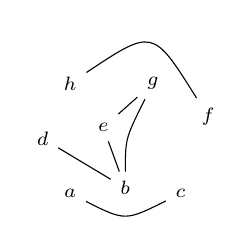
\begin{tikzpicture}[scale=.7,baseline=.5cm]
	\node (a) at (0,0) {$\scriptstyle a$};
	\node (b) at (1,.1) {$\scriptstyle b$};
	\node (c) at (2,0) {$\scriptstyle c$};
	\node (d) at (-.5,1) {$\scriptstyle d$};
	\node (e) at (.6,1.2) {$\scriptstyle e$};
	\node (h) at (0,2) {$\scriptstyle h$};
	\node (g) at (1.5,2) {$\scriptstyle g$};
	\node (f) at (2.5,1.4) {$\scriptstyle f$};
	\draw (a) .. controls (1,-.5) .. (c); 
	\draw (b) .. controls (1,1) .. (g); 
	\draw (h) .. controls (1.5,3) .. (f); 
	\draw (g) -- (e); 
	\draw (b) -- (e); 
	\draw (d) -- (b); 
\end{tikzpicture} 
\qquad \qquad
y=
\begin{tikzpicture}[scale=.7,baseline=.5cm]
	\node (a) at (0,0) {$\scriptstyle a$};
	\node (b) at (1,.1) {$\scriptstyle b$};
	\node (c) at (2,0) {$\scriptstyle c$};
	\node (d) at (-.5,1) {$\scriptstyle d$};
	\node (e) at (.6,1.2) {$\scriptstyle e$};
	\node (h) at (0,2) {$\scriptstyle h$};
	\node (g) at (1.5,2) {$\scriptstyle g$};
	\node (f) at (2.5,1.4) {$\scriptstyle f$};
	\draw (b) -- (e); 
	\draw (d) -- (b); 
\end{tikzpicture} 
$$
and let $\alpha,\beta$ be the orders $\alpha=abcdefgh$, $\beta=abdefghc$. The minimum element of $\mathcal{C}_{\alpha,x}^{\beta,y}$
is $\Lambda=(a,bde,f,g,h,c)$ (notice that indeed $x_{\Lambda}=y$ and $\alpha_{\Lambda}=\beta$). Since $\Lambda$ has $6$ parts, the graph $G_{\alpha,x}^{\beta,y}$ is build on the set $[6]=\{1,2,\ldots,6\}$.
We have 
$$G_{\alpha,x}^{\beta,y}=
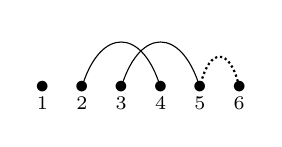
\begin{tikzpicture}[baseline=.2cm]
	\foreach \x in {1,2,3,4,5,6} 
		\node (\x) at (\x/2,0) [inner sep=-1pt] {$\bullet$};
	\node at (1/2,-.2) {$\scriptstyle 1$};
	\node at (2/2,-.2) {$\scriptstyle 2$};
	\node at (3/2,-.2) {$\scriptstyle 3$};
	\node at (4/2,-.2) {$\scriptstyle 4$};
	\node at (5/2,-.2) {$\scriptstyle 5$};
	\node at (6/2,-.2) {$\scriptstyle 6$};
	\draw (2) .. controls (2.5/2,.75) and (3.5/2,.75) .. (4); 
	\draw (3) .. controls (3.5/2,.75) and (4.5/2,.75) .. (5); 
	\draw [densely dotted,thick] (5) .. controls (5.25/2,.5) and (5.75/2,.5) .. (6); 
\end{tikzpicture} .
$$
In particular, notice that $(1,2)$ is not an edge as the element $B=(\Lambda_1\cup\Lambda_2,\Lambda_3,\dots,\Lambda_6)=(abde,f,g,h,c)\in \mathcal{C}_{\alpha,x}^{\beta,y}$.
The solid edges $(i,j)$ indicate that $ x_{B_{ij}}\ne y$, the dotted edge $(5,6)$ indicates that $ \alpha_{B_{56}}=abdefgch\ne \beta$. 
We now identify the set compositions in the interval $[\Lambda,(I)]$ with the set compositions of the interval $[(1,2,\ldots,m),(12\cdots m)]$ 
and represent $\mathcal{C}_{\alpha,x}^{\beta,y}$ via the following poset
$$
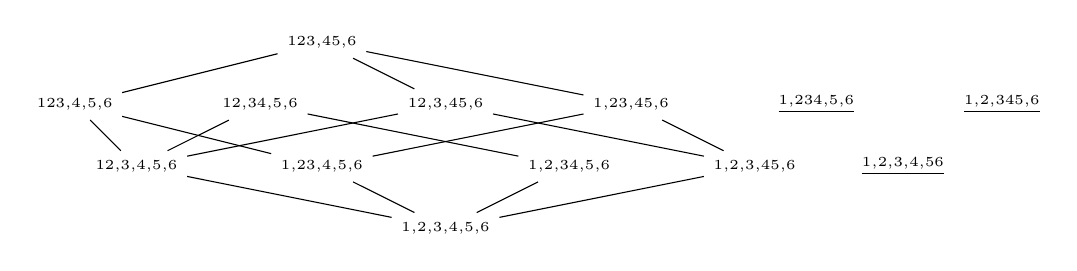
\begin{tikzpicture}[scale=1.57,baseline=.5cm]
	\node (0) at (0,0) {$\scriptscriptstyle 1,2,3,4,5,6$};
	\node (12) at (-2.5,.5) {$\scriptscriptstyle 12,3,4,5,6$};
	\node (23) at (-1,.5) {$\scriptscriptstyle 1,23,4,5,6$};
	\node (34) at (1,.5) {$\scriptscriptstyle 1,2,34,5,6$};
	\node (45) at (2.5,.5) {$\scriptscriptstyle 1,2,3,45,6$};
	\node (56) at (3.7,.5) {$\scriptscriptstyle \red{\underline{1,2,3,4,56}}$};
	\draw (0) -- (12);
	\draw (0) -- (23);
	\draw (0) -- (34);
	\draw (0) -- (45);
	\node (123) at (-3,1) {$\scriptscriptstyle 123,4,5,6$};
	\node (12_34) at (-1.5,1) {$\scriptscriptstyle 12,34,5,6$};
	\node (12_45) at (0,1) {$\scriptscriptstyle 12,3,45,6$};
	\node (234) at (3,1) {$\scriptscriptstyle \red{\underline{1,234,5,6}}$};
	\node (23_45) at (1.5,1) {$\scriptscriptstyle 1,23,45,6$};
	\node (345) at (4.5,1) {$\scriptscriptstyle \red{\underline{1,2,345,6}}$};
	\draw (12)--(123);
	\draw (12)--(12_34);
	\draw (12)--(12_45);
	\draw (23)--(123);
	\draw (23)--(23_45);
	\draw (34)--(12_34);
	\draw (45)--(23_45);
	\draw (45)--(12_45);
	\node (123_45) at (-1,1.5) {$\scriptscriptstyle 123,45,6$};
	\draw (23_45)-- (123_45);
	\draw (123)--(123_45);
	\draw (12_45)--(123_45);
\end{tikzpicture} 
$$
where the set compositions in red are the minimal compositions in $[\Lambda,(I)] \backslash \mathcal{C}_{\alpha,x}^{\beta,y}$ from Lemma~\ref{le:upperideal}.
\end{exam}

\begin{rema}
As in the example above, from now on we will identify the set compositions in the interval $[\Lambda,(I)]$ with the set compositions in the interval $[(1,2,\ldots,m),(12\cdots m)]$.
Thus, each element $A\in \mathcal{C}_{\alpha,x}^{\beta,y}$ will be viewed as the corresponding set composition $A\models[m]$.
% From Lemma~\ref{le:upperideal} we have that $A\in \mathcal{C}_{\alpha,x}^{\beta,y} $ if and only if no edge of $G_{\alpha,x}^{\beta,y}$ lies completely in a part of $A$. That is $A$ separates every edges of $G_{\alpha,x}^{\beta,y}$.
\end{rema}

For any set composition $B$ define its sign to be $sgn(B):=(-1)^{\ell (B)}$, where $\ell(B)$ is the length of $B$. We now define a sign reversing involution $\varphi\colon \mathcal{C}_{\alpha,x}^{\beta,y} \to \mathcal{C}_{\alpha,x}^{\beta,y}$, making use of auxiliary maps $\varphi _i$ for each $1\le i <m$, as follows.
Let $A=(A_1,\ldots,A_k)\in \mathcal{C}_{\alpha,x}^{\beta,y}$ and let $j$ be such that $i\in A_j$.


\begin{enonce*}{$i$-Merge} If $A_j=\{i\}$ and $(i,r)$ is not an edge of $G_{\alpha,x}^{\beta,y}$ for any $r\in A_{j+1}$, 
define
 $$ \varphi_i(A)=(A_1,\ldots,A_{j-1},\{i\}\cup A_{j+1},A_{j+2},\ldots, A_k).$$
\end{enonce*}


\begin{enonce*}{$i$-Split} If $|A_j|>1$, $i=\min(A_j)$ and \big($j=1$ or $A_{j-1}\ne\{i-1\}$ or $(i-1,i)\in G_{\alpha,x}^{\beta,y}$\big), then
 $$ \varphi_i(A)=(A_1,\ldots,A_{j-1},\{i\},A_{j}\setminus\{i\},A_{j+1},\ldots, A_k).$$
\end{enonce*}
 
\begin{enonce*}{$i$-Fix} If we do not have an $i$-merge or an $i$-split, then
 $$\varphi_i(A)=A.$$
\end{enonce*}
 
 Then the map $\varphi$ is defined as
 \begin{equation}\label{eq:involution}
 \varphi(A):=\begin{cases}
 A & \text{if $\varphi_i(A)=A$ for all $1\le i<m$,}\\
 \varphi_{i_0}(A) & \text{for $i_0=\min\big\{i:\varphi_i(A)\ne A\big\}$, otherwise.}\\
 \end{cases}
 \end{equation}

\begin{lemma}\label{le:involution}
 $\varphi\colon \mathcal{C}_{\alpha,x}^{\beta,y} \to \mathcal{C}_{\alpha,x}^{\beta,y}$ is an involution.
\end{lemma}
 
\begin{proof} Let $A\in \mathcal{C}_{\alpha,x}^{\beta,y}$. If $\varphi(A)=A$ the claim follows. Assume then that $\varphi(A)=A'\ne A$. Let $i_0=\min\big\{i:\varphi_i(A)\ne A\big\}$, and thus $A'= \varphi_{i_0}(A)$. We first assume that $A'$ is obtained from $A$ by an $i_0$-split, then $A'<A$ and thus by Lemma~\ref{le:lowerideal}, $A' \in \mathcal{C}_{\alpha,x}^{\beta,y}$. Moreover, applying an $i_0$-split to $A$ guarantees that an $(i_0-1)$-merge can not be applied to $A'$. The minimality of $i_0$ guarantees that $\varphi_i(A')=A'$ for all $i<i_0$ and $\varphi(A')=\varphi_{i_0}(A')=A$ is obtained from $A'$ by an $i_0$-merge as desired.

Now assume that $A'$ is obtained by an $i_0$-merge. This implies that no part of $A'$ contains (the vertices of) any edge of $G_{\alpha,x}^{\beta,y}$. Hence, $A' \in \mathcal{C}_{\alpha,x}^{\beta,y}$ by Lemma~\ref{le:upperideal}. Again, the minimality of $i_0$ guarantees that $\varphi_i(A')=A'$ for all $i<i_0$ and $\varphi(A')=\varphi_{i_0}(A')=A$ is obtained from $A'$ by an $i_0$-split. Finally, notice that in either case, $sgn( \varphi(A))\neq sgn(A)$ whenever $ \varphi(A)\neq A$.
\end{proof}

%%%%%%%%%%%%%%
%% PROOF OF THEOREM
%%%%%%%%%%%%%%
\subsection{Proof of Theorem~\ref{thm:antiLxP}}\label{ss:proof1} Lemma~\ref{le:involution} tells us that every element $A$ in the poset $\mathcal{C}_{\alpha,x}^{\beta,y}$ is either a fixed point, or is paired with a unique element $B\in\mathcal{C}_{\alpha,x}^{\beta,y}$ such that $B$ is a covering of $A$ or $A$ covers it. Thus, equation~\eqref{eq:anticoef} can be rewritten as:
\begin{equation}\label{eq:anticoeffix}
 c_{\alpha,x}^{\beta,y}=\sum_{\stackrel{A\in \mathcal{C}_{\alpha,x}^{\beta,y}} %\atop 
 {\varphi(A)=A}} (-1)^{\ell(A)}.
\end{equation}
This depends only on the structure of the graph $G_{\alpha,x}^{\beta,y}$, which as remarked earlier, is non-nesting. In this section we let $G:=G_{\alpha,x}^{\beta,y}$ be a non-nesting graph on the vertices $\{1,2,\ldots, m\}$ and set $\mathcal{C}(G):= \mathcal{C}_{\alpha,x}^{\beta,y}$, $c(G) := c_{\alpha,x}^{\beta,y}$. Our next task is to describe the fixed points of $\varphi\colon \mathcal{C}(G)\to \mathcal{C}(G)$ in order to resolve equation (\ref{eq:anticoeffix}). To this end, we now prove some auxiliary lemmas that show how $c(G)$ is affected by certain properties that the graph $G$ may have.

\begin{defi}\label{def:decomposible}
Let $G$ be as above. We say that $G$ is \emph{decomposible} if there exists a vertex $1\leq r<m$ such that there is no arc $(a,b)\in G$ with $a\in\{1,\dots ,r\}$ and $b\in\{r+1,\dots,m\}$.

%We say that $G$ is \emph{decomposible}{\footnote{Think of the graph $G$ as drawn on the real line. Whenever $G$ is decomposible, in the usual sense of the word, the midpoints between the vertices of $G$ tell us where the disconnectivity happens.}} if there is an integer $r$ such that $1\le \frac{2r+1}{2} \le m$ and no edge $(a,b)\in G$ such that $a\le \frac{2r+1}{2}\le b$.
\end{defi}

\begin{lemma}\label{le:decomposible}
 If $G$ is decomposible, then $c(G)=0$.
\end{lemma}

\begin{proof}
Let $r$ be as in Definition~\ref{def:decomposible}. We construct a different sign reversing involution $\psi_r\colon \mathcal{C}(G)\to \mathcal{C}(G)$ with no fixed points, and thus the claim will follow. Let $A=(A_1,\ldots,A_k)\in \mathcal{C}(G)$ and let $r\in A_j$. If $r+1\in A_j$ let 
$$
\psi_r(A_j) :=(A_1,\ldots,A_{j-1},\{\min(A_j),\ldots,r\},\{r+1,\ldots,\max(A_j)\},A_{j+1},\ldots,A_k) .
$$
Thus by Lemma~\ref{le:lowerideal}, $\psi_r(A_j) \in \mathcal{C}(G)$ since $\psi_r(A_j)$ refines $A$. If $r+1\notin A_j$ then $r+1=\min A_{j+1}$. In this case let
$$\psi_r(A)=(A_1,\ldots,A_{j-1},A_j\cup A_{j+1},A_{j+2},\ldots,A_k).$$ Since $G$ is decomposible at $r$ we see that $\psi_r(A_j) \in \mathcal{C}(G) $, as desired. It is not difficult to check that in either case, $\psi_r(\psi_r(A_j))= A_j$. This completes the proof.
% 
%Let $A=(A_1,\ldots,A_k)\in \mathcal{C}(G)$ and let $j=\max\big\{i: \min(A_i)<\frac{2r+1}{2}\big\}$.
%If $\frac{2r+1}{2}<\max(A_j)$ let
% $$\psi_r(A)=A'=(A_1,\ldots,A_{j-1},\{\min(A_j),\ldots,r\},\{r+1,\ldots,\max(A_j)\},A_{j+1},\ldots,A_k)\ne A.$$
%Lemma~\ref{le:lowerideal} guaranties that $A' \in \mathcal{C}(G)$. Now if $\frac{2r+1}{2}>\max(A_j)$, then we must have that 
%$j<k$ and $\min(A_{j+1})=r+1$. In this case we let
% $$\psi_r(A)=A'=(A_1,\ldots,A_{j-1},A_j\cup A_{j+1},A_{j+2},\ldots,A_k)\ne A.$$
%The hypothesis on $G$ and Lemma~\ref{le:upperideal} gives that $A' \in \mathcal{C}(G)$.
%We have that $\psi_r$ is a signed-reversing involution with no fixed point and all terms in equation~\eqref{eq:anticoef} cancel as desired.
\end{proof}

\begin{lemma}\label{le:shortedge}
 If $(i,i+1)\in G$ for some $1\le i<m$, then 
 $$ c(G)= c\big(G|_{\{1,\ldots, i\}}\big)\cdot c\big(G|_{\{i+1,\ldots, m\}}\big) .$$
\end{lemma}
\begin{proof} If $(i,i+1)\in G$ for some $1\le i<m$, then there is no other edge $(a,b)\in G$ with $a\le i<b$ since $G$ is non-nesting. Thus $G$ is formed by the subgraphs $G' = G|_{\{1,\ldots, i\}}$ and $G''=G|_{\{i+1,\ldots, m\}}$ together with the edge $(i,i+1)$ that connects $G'$ and $G''$. Moreover, in such case the set $\mathcal{C}(G)$ is isomorphic to $\mathcal{C}(G')\times \mathcal{C}(G'')$ since for any $A\in\mathcal{C}(G)$, $i$ and $i+1$ must be separated in $A$.
%
%This implies that
% $G$ decompose into the edge $(i,i+1)$ and two subgraphs $G' = G|_{\{1,\ldots, i\}}$ and $G''=G|_{\{i+1,\ldots, m\}}$ restricted to the vertices $\{1,\ldots,i\}$ and $\{i+1,\ldots m\}$. 
%For all $A\in \mathcal{C}(G)$ we never have $i$ and $i+1$ in the same part. In particular $\mathcal{C}(G) \cong \mathcal{C}(G')\times \mathcal{C}(G'')$.
Hence
$$ 
\begin{aligned}
c(G) &= \sum_{A\in \mathcal{C}(G)} (-1)^{\ell(A)} 
\\
&= \sum_{(A',A'')\in \mathcal{C}(G')\times \mathcal{C}(G'')} (-1)^{\ell(A')+\ell(A'')}= c\big(G|_{\{1,\ldots, i\}}\big)\cdot c\big(G|_{\{i+1,\ldots, m\}}\big) 
\end{aligned}
$$
as desired. \end{proof}

From Lemma~\ref{le:decomposible} and Lemma~\ref{le:shortedge}, we can assume from now on that $G$ is non-nesting, connected and with no short edges, i.e., edges of the form $(i,i+1)$. In particular, such $G$ must contain an edge $(1,\ell)\in G$ with $2<\ell\le m$. Moreover, if $\ell=m$ it follows that $G=\{(1,m)\}$ and the only fixed point of $\varphi$ is the set composition $A=(\{1\},\{2,\ldots,m\})$. 


Now, assume that $2<\ell<m$. Since $G$ is connected, there must be an edge
$(a,b)\in G$ such that $1<a\le \ell<b\le m$. Consider the set of edges $\big\{(a_1,b_1),\ldots,(a_n,b_n)\big\}\subseteq G$ such that $$1<a_1<a_2<\cdots<a_n\le\ell<b_1<b_2<\cdots< b_n\le m.$$
% These edges can be pictured as
%\begin{equation}\label{eq:thegraph}
%G=
%\begin{tikzpicture}[baseline=.2cm]
%	\foreach \x in {1,3,5,7,9,11,15} 
%		\node (\x) at (\x/2,0) [inner sep=-1pt] {$\bullet$};
%	\node at (1/2,-.2) {$\scriptstyle 1$};
%	\node at (2/2,-.2) {$\scriptstyle \cdots$};	
%	\node at (3/2,-.2) {$\scriptstyle a_1$};
%	\node at (4/2,-.2) {$\scriptstyle \cdots$};	
%	\node at (5/2,-.2) {$\scriptstyle a_n$};
%	\node at (6/2,-.2) {$\scriptstyle \cdots$};	
%	\node at (7/2,-.2) {$\scriptstyle \ell$};
%	\node at (8/2,-.2) {$\scriptstyle \cdots$};	
%	\node at (9/2,-.2) {$\scriptstyle b_1$};
%	\node at (10/2,-.2) {$\scriptstyle \cdots$};	
%	\node at (11/2,-.2) {$\scriptstyle b_n$};
%	\node at (13/2,-.2) {$\scriptstyle \cdots$};	
%	\node at (15/2,-.2) {$\scriptstyle m$};
%	\draw [thick] (1) .. controls (3/2,1) and (5/2,1) .. (7); 
%	\draw [densely dotted, thick] (3) .. controls (5/2,.75) and (7/2,.75) .. (9); 
%	\draw [densely dotted, thick] (5) .. controls (7/2,.75) and (9/2,.75) .. (11); 
%\end{tikzpicture} 
%\end{equation}

\begin{lemma}\label{le:nequal1} With $\big\{(a_1,b_1),\ldots,(a_n,b_n)\big\}$ as above, we have that the fixed points of $\varphi$ depend only on $(a_1,b_1)$.
\end{lemma}

\begin{proof} 
Assume that $n>1$ and that $A=(A_1,\ldots,A_k)\in \mathcal{C}(G)$ is a fixed point of $\varphi$. We have that $A_1=\{1\}$; otherwise we could perform a 1-split on $A$. Similarly, $A_2=\{2,\ldots,r\}$ and thus $ \ell\le r$; otherwise we could perform a 1-merge on $A$. Also, $\ell\le r<b_1$ as the edge $(a_1,b_1)$ can not be contained in $A_2$. Moreover, $|A_2|>2$ and $\{r+1,\ldots,m\}$ has at least two elements. Thus $A_3=\{r+1,...\}$ is nonempty. If $|A_3|>1$, then we can perform an $r+1$-split which contradicts the choice of $A$. Hence, $A_3=\{r+1\}$. Let $c=r+1$ and $A_4=\{c+1,\ldots,r'\}$. If there is no edge $(c,d)\in G$, then we would be allowed to do a $c$-merge on $A$, contradicting its choice. Thus such an edge $(c,d)$ exists. Since $G$ is non-nesting, we have $ 1<a_1\le\ell <c\le b_1<b_n<d\le m$. That is
\begin{equation}\label{eq:firstarcs}
G=
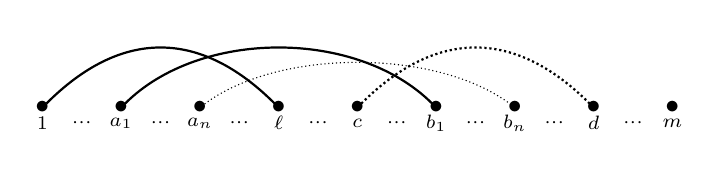
\begin{tikzpicture}[baseline=.2cm]
	\foreach \x in {1,3,5,7,9,11,13,15,17} 
		\node (\x) at (\x/2,0) [inner sep=-1pt] {$\bullet$};
	\node at (1/2,-.2) {$\scriptstyle 1$};
	\node at (2/2,-.2) {$\scriptstyle \cdots$};	
	\node at (3/2,-.2) {$\scriptstyle a_1$};
	\node at (4/2,-.2) {$\scriptstyle \cdots$};	
	\node at (5/2,-.2) {$\scriptstyle a_n$};
	\node at (6/2,-.2) {$\scriptstyle \cdots$};	
	\node at (7/2,-.2) {$\scriptstyle \ell$};
	\node at (8/2,-.2) {$\scriptstyle \cdots$};	
	\node at (9/2,-.2) {$\scriptstyle c$};
	\node at (10/2,-.2) {$\scriptstyle \cdots$};	
	\node at (11/2,-.2) {$\scriptstyle b_1$};
	\node at (12/2,-.2) {$\scriptstyle \cdots$};	
	\node at (13/2,-.2) {$\scriptstyle b_n$};
	\node at (14/2,-.2) {$\scriptstyle \cdots$};	
	\node at (15/2,-.2) {$\scriptstyle d$};
	\node at (16/2,-.2) {$\scriptstyle \cdots$};	
	\node at (17/2,-.2) {$\scriptstyle m$};
	\draw [thick] (1) .. controls (3/2,1) and (5/2,1) .. (7); 
	\draw [thick] (3) .. controls (5/2,1) and (9/2,1) .. (11); 
	\draw [densely dotted] (5) .. controls (7/2,.75) and (11/2,.75) .. (13); 
	\draw [densely dotted,thick] (9) .. controls (11/2,1) and (13/2,1) .. (15); 
\end{tikzpicture} 
 \end{equation}
Hence,
 \begin{equation}\label{eq:firstparts}
 A=\big(\{1\},\{2,\ldots,c-1\},\{c\},\{c+1,\ldots,r'\},\ldots\big)
 \end{equation}
where $\mk r'\Mk \ge \Mk d\mk$. Thus, the fixed point $\mk A\mk$ does not depend on the edges $(a_2,b_2),\ldots,(a_n,b_n)$, and the claim follows.
\end{proof}

The proof of Lemma~\ref{le:nequal1} gives us a necessary condition on the fixed points of $\varphi$.

\begin{lemma}\label{le:fixshape} Let $G$ be connected with no small edges.
 If $A\in \mathcal{C}(G)$ is a fixed point of $\varphi$, then 
 $$
 A=(\{{1}\},\{2,\ldots,x_2-1\},\{x_2\},\{x_2+1,\ldots,x_4-1\},\ldots,\{x_{2k}\},\{x_{2k}+1,\ldots,m\})
 $$
 when $\ell(A)$ is even, and
 $$
 A\Mk = \Mk (\{1\},\{2,\ldots,x_2-1\},\{x_2\},\{x_2+1,\ldots,x_4-1\},\ldots,\{x_{2k}\},\{x_{2k}+1,\ldots,m-1\},\{m\})
 $$ 
when $\ell(A)$ is odd. In each case $G$ contains, respectively, edges of the form
\begin{align*}
& \big\{(x_0,y_0),(x_1,y_1),\ldots,(x_{2k},y_{2k})\big\}\text{ with }x_0=1 \text{ and }y_{2k} = m,\text{ or},\\
 &\big\{(x_0,y_0),(x_1,y_1),\ldots,(x_{2k},y_{2k}),(x_{2k+1},y_{2k+1})\big\}\text{ with }x_0=1 \text{ and }y_{2k+1} = m
 \end{align*}
 such that 
 \begin{enumerate}[(i)]
 \item %[(i)] 
\label{lemma2.12_i} for $0\le i\le k-1$ we have $x_{2i}<x_{2i+1}\le y_{2i}<x_{2i+2}\le y_{2i+1}<y_{2i+2}$,
 \item %[(ii)] 
\label{lemma2.12_ii} there is no edge $(x,y)\in G$ such that $x_{2i}<x<x_{2i+1}$.
 \end{enumerate}
\end{lemma}

\begin{proof} 

The case where $G$ has only one edge was considered prior to Lemma~\ref{le:nequal1}. In this case, the unique fixed point is $A=(\{1\},\{2,\ldots,m\})$. 

If $G$ has more than one edge,
Lemma~\ref{le:nequal1} tells us that the fixed points of $\varphi$ depend only on edges of the form
$(1,\ell)$, $(a_1,b_1)$ and the possible $(c,d)$ as in equation~\eqref{eq:firstarcs}. If there is no such edge $(c,d)$, then 
$G=\big\{(1,\ell),(a_1,b_1),\ldots,(a_n,b_n)\big\}$, where $1<a_j\le \ell<b_j\le m$ and $b_n=m$.
For $n>1$, we have seen in the proof of Lemma~\ref{le:nequal1} that if there is no arc $(c,d)\in G$ with $ 1<a_1<a_n \le\ell <c\le b_1<b_n<d\le m$, then there is no fixed point of $\varphi$. 
If $n=1$, then $G=\big\{(1,\ell),(a,m)\big\}$ for $1<a\le \ell<m$. Our analysis shows that in this case there is a unique fixed point $A=(\{1\},\{2,\ldots,m-1\},\{m\})$. Here $\ell(A)=3$ is odd, $k=0$ and 
again all the conditions of the lemma are satisfied.

Assume now that $G$ has an edge $(c,d)$ as in equation~\eqref{eq:firstarcs}. Since for $j>1$, the edges $(a_j,b_j)$ do not play a role 
in our analysis of the fixed point of $\varphi$, we can omit them. Let $(a,b)=(a_1,b_1)$ and consider the set of arcs $\big\{(c_1,d_1),\ldots,(c_n,d_n)\big\}\subseteq G$ such that $\ell<c_j\le b<d_j\le m$. We now have
\begin{equation}\label{eq:nextarcs}
G=
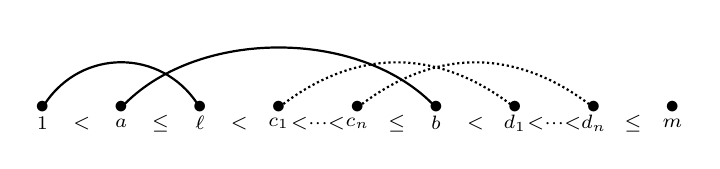
\begin{tikzpicture}[baseline=.2cm]
	\foreach \x in {1,3,5,7,9,11,13,15,17} 
		\node (\x) at (\x/2,0) [inner sep=-1pt] {$\bullet$};
	\node at (1/2,-.2) {$\scriptstyle 1$};
	\node at (2/2,-.2) {$\scriptstyle <$};	
	\node at (3/2,-.2) {$\scriptstyle a$};
	\node at (4/2,-.2) {$\scriptstyle \le$};	
	\node at (5/2,-.2) {$\scriptstyle \ell$};
	\node at (6/2,-.2) {$\scriptstyle <$};	
	\node at (7/2,-.2) {$\scriptstyle c_1$};
	\node at (8/2,-.2) {$\scriptstyle <\cdots <$};	
	\node at (9/2,-.2) {$\scriptstyle c_n$};
	\node at (10/2,-.2) {$\scriptstyle \le$};	
	\node at (11/2,-.2) {$\scriptstyle b$};
	\node at (12/2,-.2) {$\scriptstyle <$};	
	\node at (13/2,-.2) {$\scriptstyle d_1$};
	\node at (14/2,-.2) {$\scriptstyle <\cdots <$};	
	\node at (15/2,-.2) {$\scriptstyle d_n$};
	\node at (16/2,-.2) {$\scriptstyle \le$};	
	\node at (17/2,-.2) {$\scriptstyle m$};
	\draw [thick] (1) .. controls (2/2,.75) and (4/2,.75) .. (5); 
	\draw [thick] (3) .. controls (5/2,1) and (9/2,1) .. (11); 
	\draw [densely dotted,thick] (7) .. controls (9/2,.75) and (11/2,.75) .. (13); 
	\draw [densely dotted,thick] (9) .. controls (11/2,.75) and (13/2,.75) .. (15); 
\end{tikzpicture} 
 \end{equation}
For each $1\le j<n-1$, a potential fixed point according to Equation~\eqref{eq:firstparts} would need to be of the form
\begin{equation}\label{eq:startfixpoint}
 A=(\{1\},\{2,\ldots,c_{j}-1\},\{c_{j}\},\{c_{j}+1,\ldots,r\},\{r+1,\ldots\},\ldots)
 \end{equation}
 where $d_j\le r<d_{j+1}$. The second inequality comes from the fact that we are not allowed to have $c_{j+1}$ and $d_{j+1}$ in the same part.
Hence if $A$ is a fixed point it must have the form described in Equation~\eqref{eq:startfixpoint} and we must have
 $$\big\{(x_0,y_0),(x_1,y_1),(x_2,y_2),\ldots\big\}=\big\{(1,\ell),(a,b),(c_j,d_j)\ldots\big\}\subseteq G,$$
where $ 1<a \le\ell <c_j \le b <d_j$ and there is no edge $(x,y)\in G$ such that $1<x<a$. The remaining structure of the fixed point in Equation~\eqref{eq:startfixpoint}
depends only on the structure of the smaller graph $G|_{\{c_j,\ldots,m\}}$. The result then follows by induction on the size of $G$.
\end{proof}


Now that we have a better understanding of the possible structure of the fixed points of $\varphi$, it may appear that there are many possibilities.
It turns out that there could be at most two fixed points of different parity. 
%To show that we will need a little lemma about graph $G$ with no nesting.

